\chapter{Software}
This chapter contains the design choices and an explanation of the different design blocks.

\section{CDU}
\subsection{General Description}
The software on the microcontroller governs the sensor communication, the PC communication and the memory. The hierarchy of software can be seen on the class diagram in figure ~\ref{fig:cduclassd}. The software is composed of a main "while(1)" loop and an interrupt routine. Messages are composed in the main while messages are sent using the interrupt routine. This means that the message is sent using the clock tied to the routine. A timer governs when to interrupt.\\

\begin{figure}[H]
\centering
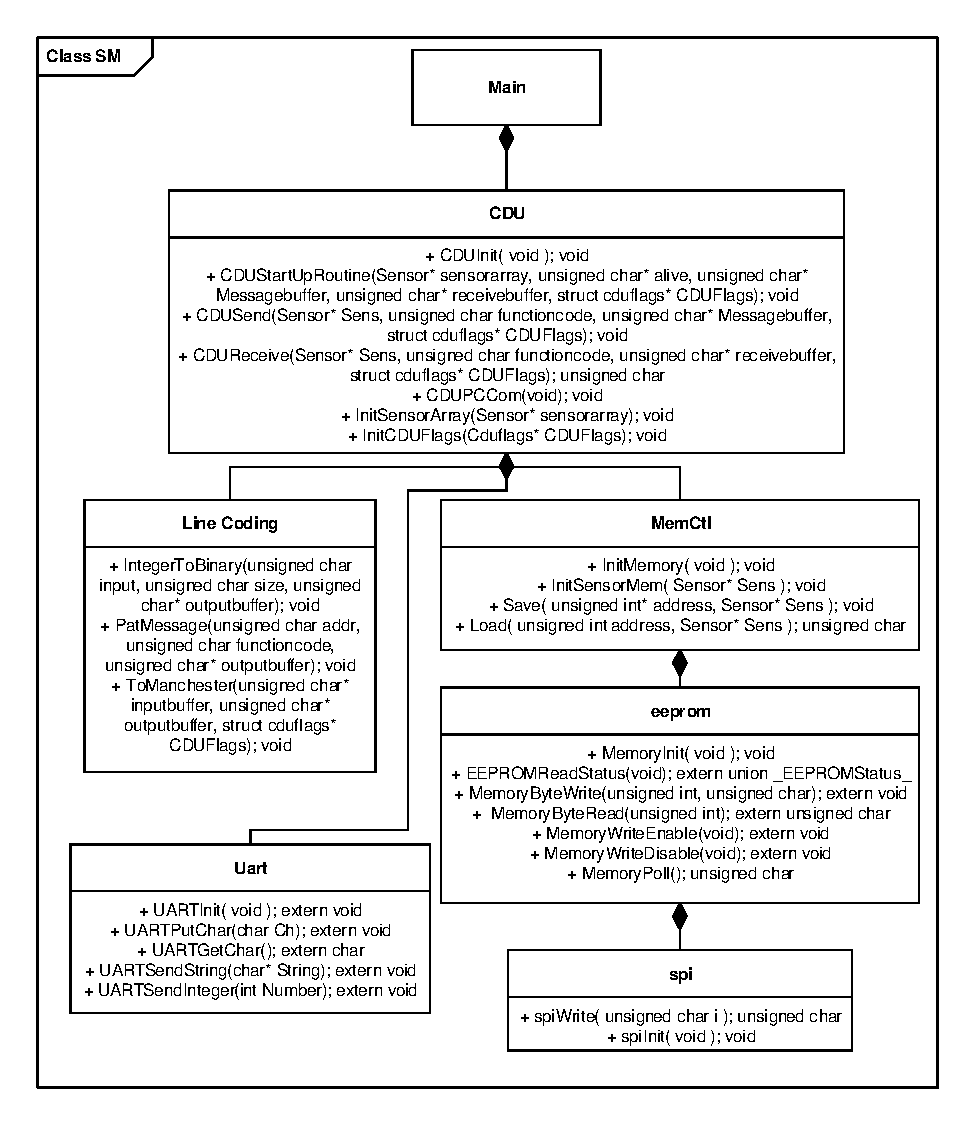
\includegraphics[scale=0.8]{billeder/CDUClassDiagramme}
\label{fig:cduclassd}
\caption{CDU Class diagram}
\end{figure}
\subsection{Module Responsibility}
Each module from the figure ~\ref{fig:cduclassd} has a different responsibility. These will be described here.
\subsubsection{CDU}
The responsibility of the CDU block is to function as an API layer. It contains Init functions, a startup routine, a send and receive function and lastly a function for PC communication. The CDU block contains everything needed to write the application layer of this project.\\
\subsubsection{Line Coding}
The line coding block contains everything needed to create messages for this project. It is used by the CDU block in the startup routine and the send function.
\subsubsection{MemCtl}
The MemCtl or Memory Control block contains the functions to initiate memory as well as save and load memory. Load is used by the PC communication function while save is intented to be used in the receive function. 
\subsubsection{eeprom}
The eeprom block handles all the hardware and timing parts of memory as well as the actual write and read functions. Write is used by the save function and read is used by the load function.
\subsubsection{spi}
The spi block is a driver block for spi communication.
\subsubsection{Uart}
The Uart block is a driver block for uart communication.

\subsection{Setup}
The setup is handled by the init function. The registers are described in this subsection.
\subsubsection{General Registers}
The general registers of the microcontroller handles general purpose pins and clock setups. The clock setup register is called "OSCCON" and are set to the following settings: "0x2200". This setting means we get a primary clock of 4 MHz with no clock division. The setup from the datasheet is found in figure ~\ref{fig:clocksetup}.\\
\begin{figure}[H]
\centering
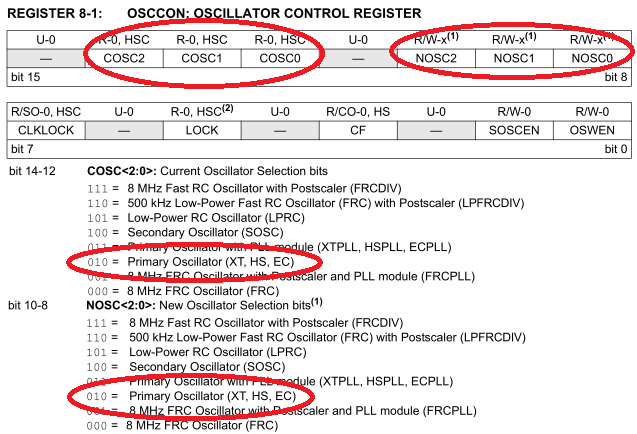
\includegraphics[width=1\textwidth]{billeder/clocksetup}
\label{fig:clocksetup}
\caption{CDU Clock Setup from datasheet}
\end{figure}
To setup the general purpose pins the registers TRISA, TRISB, TRISD and TRISF are used. By writing to TRISA the PORT A pins are controlled. If a pin is set to 1 it is an input pin otherwise it is an output pin. We setup PIN A4, A7, F4 and G7 for input. The rest for output. The full pinout table is explained in the hardware chapter of design and implementation.
\subsubsection{Timer}
In order to setup the timer we need 4 registers: "IPC0, T1CON, IFS0 and IEC0". IPC0 is used to setup interrupt priority. T1CON is the Timer 1 control register. IFS0 contains the interrupt flag tied to timer 1. IEC0 enables interrupt on timer1. The setup from the datasheet is found in figure ~\ref{fig:timersetup}.\\
\begin{figure}[H]
\centering
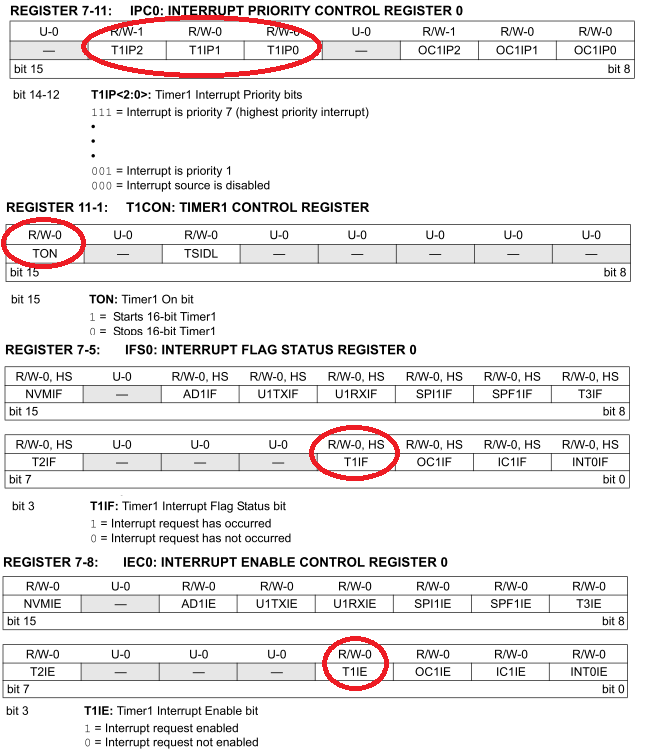
\includegraphics[width=1\textwidth]{billeder/timersetup}
\label{fig:timersetup}
\caption{CDU Timer1 Setup from datasheet}
\end{figure}
We use interrupt priority 5.\\
To control when the timer interrupts we choose the value of PR1 (timer counter register). With the value 0xC8 or 200 we get a 20 kHz interrupt.
\subsubsection{SPI}
SPI is controlled by two registers: "SPI2CON and SPI2STAT" A control and a status register. The setup for SPI1 from the datasheet is found in figure ~\ref{fig:spisetup}. SPI2 is setup the same way but the registers are not included in the datasheet.\\
\begin{figure}[H]
\centering
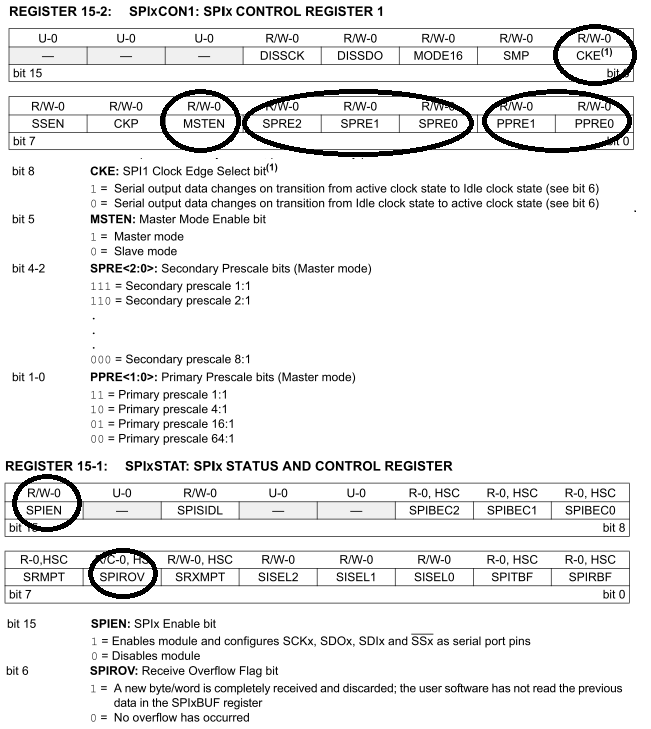
\includegraphics[width=1\textwidth]{billeder/spisetup}
\label{fig:spisetup}
\caption{CDU SPI Setup from datasheet}
\end{figure}
We use primary prescaler 1:1, secondary prescaler 2:1, CKE clock select set to 1 and master enable. SPI is enabled and the overflow flag is reset.
\subsubsection{UART}
The UART is set using the U2MODE and U2STA registers. We use setup found in figure ~\ref{fig:uartsetp}.\\
\begin{table}[H]
    \begin{tabular}{|l l|}
    \hline
    Baud rate    & : 38400 \\ \hline
    Data bit     & : 8    \\ \hline
    Parity       & : None \\ \hline
    Stop bit     & : 1    \\ \hline
    Flow control & : None \\ \hline
    \end{tabular}
    \label{fig:uartsetp}
    \caption{UART setup}
\end{table}

\subsection{Variables:}
The global variables in the CDU includes 2 structs. These 2 structs will be shown in their own table.
\begin{table}[H]
\begin{tabular}{|l|p{10cm}|}
\hline
\cellcolor[gray]{0.8}\textbf{Variable} &\cellcolor[gray]{0.8} \textbf{Description}\\ \hline
\texttt{comflag} & This varible(flag) determines whether a message is written on the bus.\\ 
\hline
\texttt{msgflag} & This varible(flag) determines whether a message is ready to be written on the bus.\\ 
\hline
\texttt{clk$\_$flag} & This varible(flag) determines whether to put a low or high out on the bus while not communicating.\\ 
\hline
\texttt{recvflag} & This varible(flag) determines whether a message has been received on the bus.\\ 
\hline
\texttt{enableflag} & This varible(flag) determines when a transmission can be written on the bus.\\ 
\hline
\end{tabular}
\label{tab:structcduflags}
\caption{Struct CDUFlags}
\end{table}

\begin{table}[H]
\begin{tabular}{|l|p{10cm}|}
\hline
\cellcolor[gray]{0.8}\textbf{Variable} &\cellcolor[gray]{0.8} \textbf{Description}\\ \hline
\texttt{Address} & This variable contains the address of the sensor node.\\ 
\hline
\texttt{Data} & This variable contains the data of the sensor node.\\ 
\hline
\texttt{Year} & This variable contains the current year.\\ 
\hline
\texttt{Day} & This variable contains the current day.\\ 
\hline
\texttt{Hour} & This variable contains the current hour.\\ 
\hline
\texttt{Minute} & This variable contains the current minute.\\ 
\hline
\texttt{Errors} & This variable contains the errors explained in the protocol section of the architecture document.\\ 
\hline
\texttt{Type} & This variable contains the type of the sensor node.\\ 
\hline
\end{tabular}
\label{tab:structsensor}
\caption{Struct Sensor}
\end{table}

\begin{table}[H]
\begin{tabular}{|l|p{10cm}|}
\hline
\cellcolor[gray]{0.8}\textbf{Variable} &\cellcolor[gray]{0.8} \textbf{Description}\\ \hline
\texttt{message} & The array will contain messages the are to be written to the bus.\\ 
\hline
\texttt{response} & The array will contain messages that have been read from the bus.\\ 
\hline
\texttt{alive} & The array contains values depending if a sensor is alive or not.\\ 
\hline
\texttt{loopcounter} & This variable(counter) is used for writing to the bus.\\ 
\hline
\texttt{recvcounter} & This variable(counter) is used for reading from the bus.\\ 
\hline
\texttt{waitclock} & This variable(counter) is used for delaying when in between writing to the bus and reading from the bus.\\ 
\hline
\texttt{addresscounter} & This variable(counter) is used for placing the point in memory in the right place.\\ 
\hline
\texttt{maincounter} & This variable(counter) is used for delaying in between transmission sequences.\\ 
\hline
\end{tabular}
\label{tab:globalvar}
\caption{Global variables}
\end{table}


\subsection{Function descriptions:}

\begin{table}[H]
\begin{tabular}{l p{12.5cm}}
\multicolumn{2}{l}{\texttt{\textcolor{blue}{void} CDUInit( \texttt{\textcolor{blue}{void}})}} \\
\hline
Description:& The function is used to Initiate the whole CDU. The proper register settings for timer, uart and spi are set. Arrays and structs are initialised.\\
Parameters:&none\\
Return value:&none\\
\end{tabular}
\end{table}

\begin{table}[H]
\begin{tabular}{l p{12.5cm}}
\multicolumn{2}{p{15cm}}{\texttt{\textcolor{blue}{void} IntegerToBinary( \texttt{\textcolor{blue}{unsigned char} input, \textcolor{blue}{unsigned char} size, \textcolor{blue}{unsigned char*} outputbuffer  }) } } \\
\hline
Description:& The function is used convert an integer to a binary array.\\
Parameters:&\texttt{\textcolor{blue}{unsigned char} input}\\
&\texttt{\textcolor{blue}{unsigned char} size}\\
&\texttt{\textcolor{blue}{unsigned char*} outputbuffer}\\
Return value:&none\\
\end{tabular}
\end{table}

\begin{table}[H]
\begin{tabular}{l p{12.5cm}}
\multicolumn{2}{p{15cm}}{\texttt{\textcolor{blue}{void} PatMessage( \texttt{\textcolor{blue}{unsigned char} addr, \textcolor{blue}{unsigned char} functioncode, \textcolor{blue}{unsigned char*} outputbuffer  }) } } \\
\hline
Description:& The function is used create a message from the start code, an address and a function code. This is put into the outputbuffer.\\
Parameters:&\texttt{\textcolor{blue}{unsigned char} addr}\\
&\texttt{\textcolor{blue}{unsigned char} functioncode}\\
&\texttt{\textcolor{blue}{unsigned char*} outputbuffer}\\
Return value:&none\\
\end{tabular}
\end{table}

\begin{table}[H]
\begin{tabular}{l p{12.5cm}}
\multicolumn{2}{p{15cm}}{\texttt{\textcolor{blue}{void} ToManchester( \texttt{\textcolor{blue}{unsigned char*} inputbuffer, \textcolor{blue}{unsigned char*} outputbuffer, \textcolor{blue}{Cduflags*} CDUFlags  }) } } \\
\hline
Description:& The function is used convert the message contained in the inputbuffer to manchester coding and put it in the outputbuffer. The outputbuffer must be twice the size of the inputbuffer. The cduflags struct contains flags to signal when a message has been put into the outputbuffer.\\
Parameters:&\texttt{\textcolor{blue}{unsigned char*} inputbuffer}\\
&\texttt{\textcolor{blue}{unsigned char*} outputbuffer}\\
&\texttt{\textcolor{blue}{Cduflags*} CDUFlags}\\
Return value:&none\\
\end{tabular}
\end{table}

\begin{table}[H]
\begin{tabular}{l p{12.5cm}}
\multicolumn{2}{l}{\texttt{\textcolor{blue}{void} InitSensorArray( \texttt{\textcolor{blue}{Sensor*} sensorarray})}} \\
\hline
Description:& The function is used to Initiate the sensorarray with addresses and values. Addresses are assigned from 1 to 15. The rest is instantiated to zero.\\
Parameters:&\texttt{\textcolor{blue}{Sensor*} sensorarray}\\
Return value:&none\\
\end{tabular}
\end{table}

\begin{table}[H]
\begin{tabular}{l p{12.5cm}}
\multicolumn{2}{l}{\texttt{\textcolor{blue}{void} InitCDUFlags( \texttt{\textcolor{blue}{Cduflags*} CDUFlags})}} \\
\hline
Description:& The function is used to Initiate the cduflags in the Cduflags struct to zero.\\
Parameters:&\texttt{\textcolor{blue}{Sensor*} sensorarray}\\
Return value:&none\\
\end{tabular}
\end{table}

\begin{table}[H]
\begin{tabular}{l p{12.5cm}}
\multicolumn{2}{p{15cm}}{\texttt{\textcolor{blue}{void} CDUStartUpRoutine( \texttt{\textcolor{blue}{Sensor*} sensorarray, \textcolor{blue}{unsigned char*} alive, \textcolor{blue}{unsigned char*} Messagebuffer, \textcolor{blue}{unsigned char*} receivebuffer, \textcolor{blue}{Cduflags*} CDUFlags})}} \\
\hline
Description:& The function is used to send messages with the GETINFO function code to every sensor in the sensorarray. If a response has been received, the type is stored in the relevant sensor struct in the sensorarray. The alive is updated with the responding sensor.\\
Parameters:&\texttt{\textcolor{blue}{Sensor*} sensorarray}\\
&\texttt{\textcolor{blue}{unsigned char*} alive}\\
&\texttt{\textcolor{blue}{unsigned char*} Messagebuffer}\\
&\texttt{\textcolor{blue}{unsigned char*} receivebuffer}\\
&\texttt{\textcolor{blue}{Cduflags*} CDUFlags}\\
Return value:&none\\
\end{tabular}
\end{table}

\begin{table}[H]
\begin{tabular}{l p{12.5cm}}
\multicolumn{2}{p{15cm}}{\texttt{\textcolor{blue}{void} CDUSend( \texttt{\textcolor{blue}{Sensor*} Sens, \textcolor{blue}{unsigned char} functioncode, \textcolor{blue}{unsigned char*} Messagebuffer, \textcolor{blue}{Cduflags*} CDUFlags})}} \\
\hline
Description:& The function is used to send messages with the function code to the sensor inserted. The cduflags struct is used to poll on when to send and to set the comflag. if a function code larger than 15 is inserted the function sends out function code 0 which will result in an error on the sensor node side.\\
Parameters:&\texttt{\textcolor{blue}{Sensor*} sensorarray}\\
&\texttt{\textcolor{blue}{unsigned char} functioncode}\\
&\texttt{\textcolor{blue}{unsigned char*} Messagebuffer}\\
&\texttt{\textcolor{blue}{Cduflags*} CDUFlags}\\
Return value:&none\\
\end{tabular}
\end{table}

\begin{table}[H]
\begin{tabular}{l p{12.5cm}}
\multicolumn{2}{p{15cm}}{\texttt{\textcolor{blue}{unsigned char} CDUReceive( \texttt{\textcolor{blue}{Sensor*} Sens, \textcolor{blue}{unsigned char} functioncode, \textcolor{blue}{unsigned char*} receivebuffer, \textcolor{blue}{Cduflags*} CDUFlags})}} \\
\hline
Description:& The function is used to receive messages from the receivebuffer and verify address and function code. If the proper address and function code is received data or type is stored in the relevant sensor struct. If verification fails it returns 0. If everything went as expected a 1 is returned. 2 is returned if the function code is larger than 15.\\
Parameters:&\texttt{\textcolor{blue}{Sensor*} sensorarray}\\
&\texttt{\textcolor{blue}{unsigned char} functioncode}\\
&\texttt{\textcolor{blue}{unsigned char*} receivebuffer}\\
&\texttt{\textcolor{blue}{Cduflags*} CDUFlags}\\
Return value:&\texttt{\textcolor{blue}{unsigned char} errors}\\
\end{tabular}
\end{table}

\subsection{Flowcharts}
\begin{figure}[H]
\centering
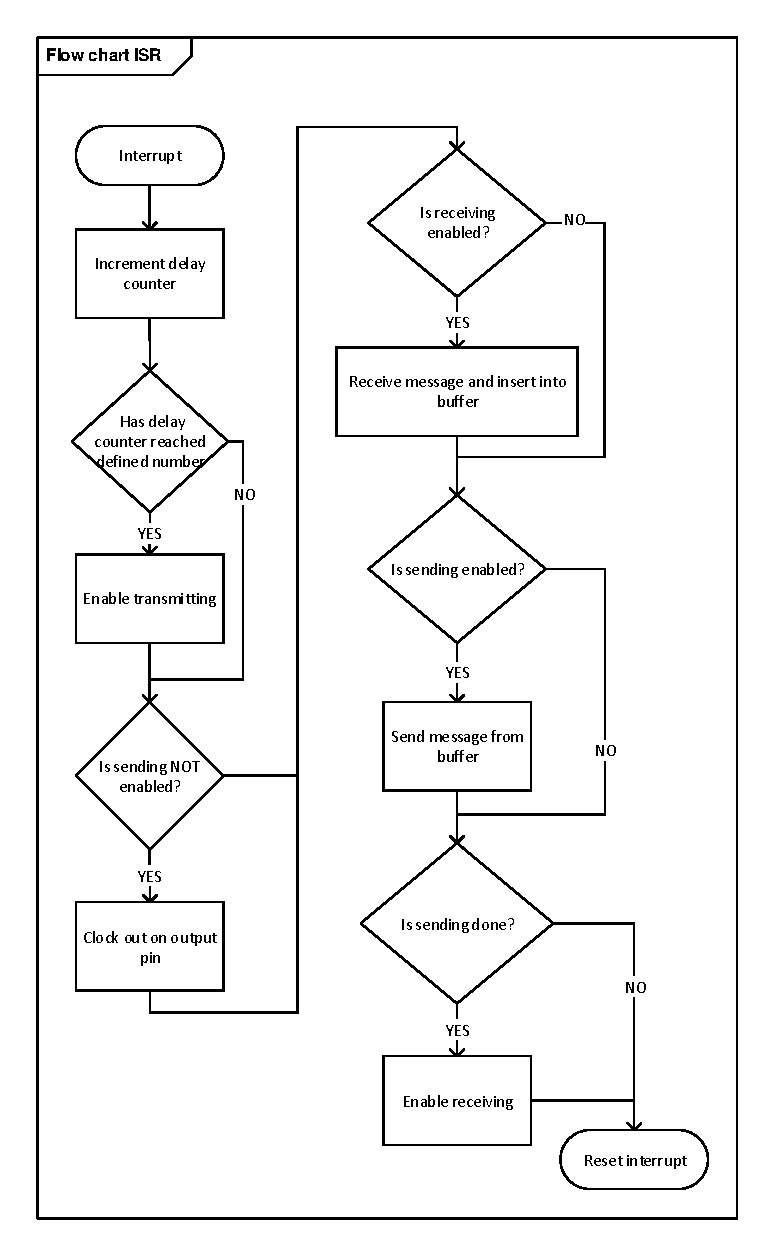
\includegraphics[width=1\textwidth]{billeder/isrflowchart}
\label{fig:isrflowchart}
\caption{CDU Interrupt service routine flowchart}
\end{figure}

\subsection{Memory Slot allocation}
\begin{figure}[H]
\centering
\includegraphics[scale=1]{billeder/memoryslots}
\label{fig:memoryslots}
\caption{CDU memory slots}
\end{figure}

\section{Sensor node}